% \section[KG-based IR]{KG-based Information Retrieval}

% \begin{frame}{Evaluation corpus contrcution}

%     \begin{figure} [H]
%         \begin{center}
%             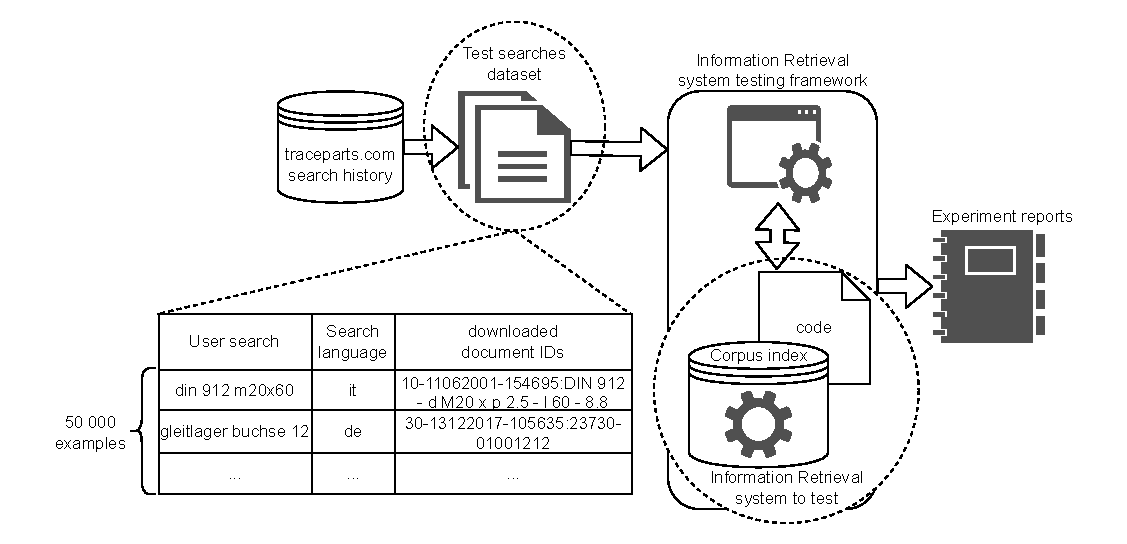
\includegraphics[scale=0.55]{images/tp-search-expe-setting.pdf} 
%             \caption{Experiments Protocol.} 
%         \end{center}
%     \end{figure}

% \end{frame}

% \begin{frame}{Evaluation metrics}

%     \begin{itemize}
%         \item Mean Average Precision at k (MAP@k): 
%         \begin{itemize}
%             \item A sliding (or growing) precision window, averaged over a set of query examples.
%             \item Ranges from $0$ to $1$ ($1$ is the best value).
%             \item Gives information about the amount and positions of positive results in the k first ones.
%         \end{itemize}
%         \item Binary Mean at k (BM@k):
%         \begin{itemize}
%             \item Binary average over a set of query examples.
%             \item Ranges from $0$ to $1$ ($1$ is the best value).
%             \item Provides information about the amount of queries with a positive result in the k first ones.
%             \item Does not give any detail on the positive result position.
%         \end{itemize}
%     \end{itemize}

% \end{frame}

% \begin{frame}{Text-based system (baseline)}

%     \begin{figure} [H]
%         \begin{center}
%             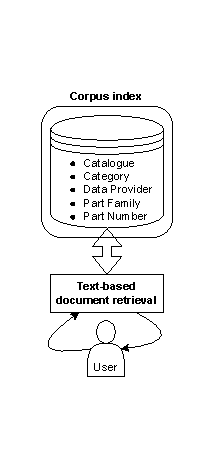
\includegraphics[scale=1]{images/tp-expe-text-based-sys.pdf} 
%             \caption{Text-based system (baseline)} 
%         \end{center}
%     \end{figure}

% \end{frame}

% \begin{frame}{Text-based system (baseline) results}

%     \begin{table}[htbp]
%         \begin{center}
%         \small
%         \begin{tabular}{c|cc|}
%             \toprule
%             \multicolumn{1}{l}{}               & \multicolumn{2}{c}{\textbf{\begin{tabular}[c]{@{}c@{}}Text-based\\ system (baseline)\end{tabular}}} \\ \cmidrule(lr){2-3}
%             \multicolumn{1}{c|}{\textbf{@k $\downarrow$}}    & \multicolumn{1}{c}{\textbf{MAP@k}} & \textbf{BM@k} \\ \cmidrule(lr){2-3}
%             \multicolumn{1}{c|}{\textbf{@5}}   & \multicolumn{1}{c}{0.061}          & 0.114       \\ 
%             \multicolumn{1}{c|}{\textbf{@25}}  & \multicolumn{1}{c}{0.064}          & 0.148       \\ 
%             \multicolumn{1}{c|}{\textbf{@50}}  & \multicolumn{1}{c}{0.064}          & 0.157       \\ 
%             \multicolumn{1}{c|}{\textbf{@100}} & \multicolumn{1}{c}{0.064}          & 0.161       \\ 
%             \multicolumn{1}{c|}{\textbf{@350}} & \multicolumn{1}{c}{0.064}          & 0.164      \\ \bottomrule
%         \end{tabular}
%         \caption{
%             Text-based system (baseline) results for different k values.
%         }\label{tab:comp-text-concept-kg}
%     \end{center}
%     \end{table} 

% \end{frame}


\begin{frame}{Knowledge Graph and ontology}

    Knowledge Graph (Hogan et. al. 2021):
    \emph{a knowledge graph is a graph of data intended to accumulate and convey knowledge of the real world, whose nodes represent entities of interest and whose edges represent relations between these entities.}
    % \emph{a knowledge graph is a graph of data intended to accumulate and convey knowledge of the real world, whose nodes represent entities of interest and whose edges represent relations between these entities. The graph of data (aka. data graph) conforms to a graph-based data model, which may be a directed edge-labelled graph, a property graph, etc. By knowledge, we refer to something that is known.}
    
    Ontology (Hogan et. al. 2021):
    \emph{In the context of computing, an ontology is then a concrete, formal representation of what terms mean within the scope in which they are used (e.g., a given domain).}

    \begin{center}
        In our work, we consider an ontology a particular component of a Knowledge Graph
    \end{center}
    
\end{frame}

\begin{frame}{Our approach based on a Knowledge Graph}

    \begin{figure} [H]
        \begin{center}
            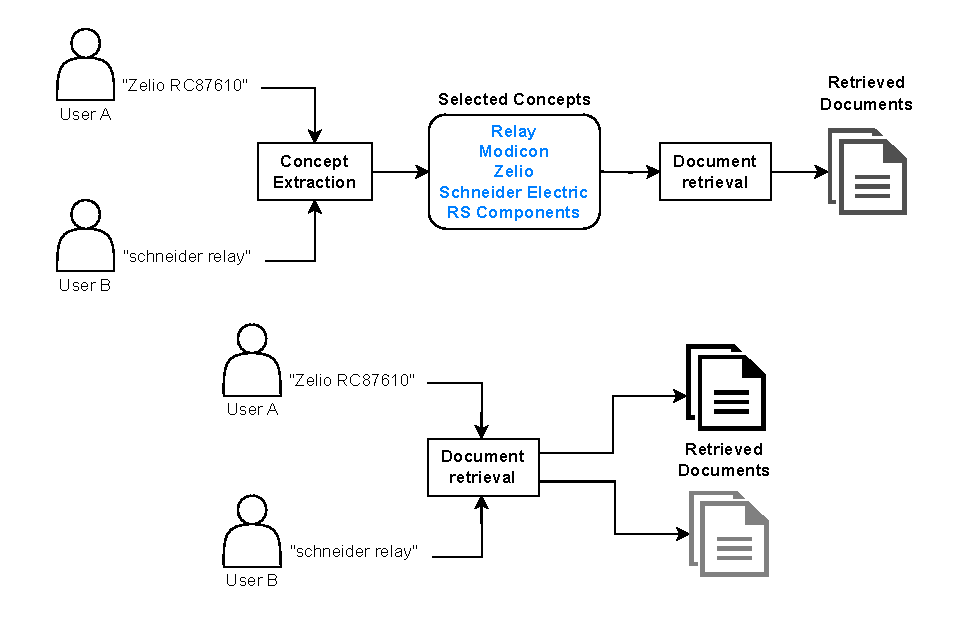
\includegraphics[scale=0.6]{images/text-vs-concept-based-search.pdf} 
            \caption{Text-based vs concept-based search.} 
        \end{center}
    \end{figure}

\end{frame}